\documentclass{article}\usepackage[]{graphicx}\usepackage[]{color}
%% maxwidth is the original width if it is less than linewidth
%% otherwise use linewidth (to make sure the graphics do not exceed the margin)
\makeatletter
\def\maxwidth{ %
  \ifdim\Gin@nat@width>\linewidth
    \linewidth
  \else
    \Gin@nat@width
  \fi
}
\makeatother

\definecolor{fgcolor}{rgb}{0.345, 0.345, 0.345}
\newcommand{\hlnum}[1]{\textcolor[rgb]{0.686,0.059,0.569}{#1}}%
\newcommand{\hlstr}[1]{\textcolor[rgb]{0.192,0.494,0.8}{#1}}%
\newcommand{\hlcom}[1]{\textcolor[rgb]{0.678,0.584,0.686}{\textit{#1}}}%
\newcommand{\hlopt}[1]{\textcolor[rgb]{0,0,0}{#1}}%
\newcommand{\hlstd}[1]{\textcolor[rgb]{0.345,0.345,0.345}{#1}}%
\newcommand{\hlkwa}[1]{\textcolor[rgb]{0.161,0.373,0.58}{\textbf{#1}}}%
\newcommand{\hlkwb}[1]{\textcolor[rgb]{0.69,0.353,0.396}{#1}}%
\newcommand{\hlkwc}[1]{\textcolor[rgb]{0.333,0.667,0.333}{#1}}%
\newcommand{\hlkwd}[1]{\textcolor[rgb]{0.737,0.353,0.396}{\textbf{#1}}}%
\let\hlipl\hlkwb

\usepackage{framed}
\makeatletter
\newenvironment{kframe}{%
 \def\at@end@of@kframe{}%
 \ifinner\ifhmode%
  \def\at@end@of@kframe{\end{minipage}}%
  \begin{minipage}{\columnwidth}%
 \fi\fi%
 \def\FrameCommand##1{\hskip\@totalleftmargin \hskip-\fboxsep
 \colorbox{shadecolor}{##1}\hskip-\fboxsep
     % There is no \\@totalrightmargin, so:
     \hskip-\linewidth \hskip-\@totalleftmargin \hskip\columnwidth}%
 \MakeFramed {\advance\hsize-\width
   \@totalleftmargin\z@ \linewidth\hsize
   \@setminipage}}%
 {\par\unskip\endMakeFramed%
 \at@end@of@kframe}
\makeatother

\definecolor{shadecolor}{rgb}{.97, .97, .97}
\definecolor{messagecolor}{rgb}{0, 0, 0}
\definecolor{warningcolor}{rgb}{1, 0, 1}
\definecolor{errorcolor}{rgb}{1, 0, 0}
\newenvironment{knitrout}{}{} % an empty environment to be redefined in TeX

\usepackage{alltt}
\usepackage[sc]{mathpazo}
\renewcommand{\sfdefault}{lmss}
\renewcommand{\ttdefault}{lmtt}
\usepackage[T1]{fontenc}
\usepackage{geometry}
\geometry{verbose,tmargin=2.5cm,bmargin=2.5cm,lmargin=2.5cm,rmargin=2.5cm}
\setcounter{secnumdepth}{2}
\setcounter{tocdepth}{2}
\usepackage[unicode=true,pdfusetitle,
 bookmarks=true,bookmarksnumbered=true,bookmarksopen=true,bookmarksopenlevel=2,
 breaklinks=false,pdfborder={0 0 1},backref=false,colorlinks=false]
 {hyperref}
\hypersetup{
 pdfstartview={XYZ null null 1}}

\makeatletter
%%%%%%%%%%%%%%%%%%%%%%%%%%%%%% User specified LaTeX commands.
\renewcommand{\textfraction}{0.05}
\renewcommand{\topfraction}{0.8}
\renewcommand{\bottomfraction}{0.8}
\renewcommand{\floatpagefraction}{0.75}

\makeatother
\IfFileExists{upquote.sty}{\usepackage{upquote}}{}
\begin{document}








The results below are generated from an R script.

\begin{knitrout}
\definecolor{shadecolor}{rgb}{0.969, 0.969, 0.969}\color{fgcolor}\begin{kframe}
\begin{alltt}
\hlkwd{setwd}\hlstd{(}\hlstr{"~/GitHub/MMSS_311_2"}\hlstd{)}

\hlcom{# Q1a) A vector with the numbers 1-5 in order }
\hlstd{a} \hlkwb{<-} \hlkwd{c}\hlstd{(}\hlnum{1}\hlstd{,}\hlnum{2}\hlstd{,}\hlnum{3}\hlstd{,}\hlnum{4}\hlstd{,}\hlnum{5}\hlstd{)}

\hlcom{# Q1b) A scalar named Mindy that takes the value 12}
\hlstd{Mindy} \hlkwb{<-} \hlnum{12}

\hlcom{# Q1c) A 2�3 matrix with the numbers 1-6 in order by rows }
\hlstd{b} \hlkwb{<-} \hlkwd{c}\hlstd{(}\hlnum{1}\hlstd{,}\hlnum{2}\hlstd{,}\hlnum{3}\hlstd{,}\hlnum{4}\hlstd{,}\hlnum{5}\hlstd{,}\hlnum{6}\hlstd{)}
\hlkwd{matrix}\hlstd{(b,}\hlnum{2}\hlstd{,}\hlnum{3}\hlstd{,}\hlnum{TRUE}\hlstd{)}
\end{alltt}
\begin{verbatim}
##      [,1] [,2] [,3]
## [1,]    1    2    3
## [2,]    4    5    6
\end{verbatim}
\begin{alltt}
\hlcom{# Q1d) A 2�3 matrix with the numbers 1-6 in order by columns }
\hlkwd{matrix}\hlstd{(b,}\hlnum{2}\hlstd{,}\hlnum{3}\hlstd{)}
\end{alltt}
\begin{verbatim}
##      [,1] [,2] [,3]
## [1,]    1    3    5
## [2,]    2    4    6
\end{verbatim}
\begin{alltt}
\hlcom{# Q1e) A 10�10 matrix of 1's }
\hlkwd{matrix}\hlstd{(}\hlnum{1}\hlstd{,}\hlnum{10}\hlstd{,}\hlnum{10}\hlstd{)}
\end{alltt}
\begin{verbatim}
##       [,1] [,2] [,3] [,4] [,5] [,6] [,7] [,8] [,9] [,10]
##  [1,]    1    1    1    1    1    1    1    1    1     1
##  [2,]    1    1    1    1    1    1    1    1    1     1
##  [3,]    1    1    1    1    1    1    1    1    1     1
##  [4,]    1    1    1    1    1    1    1    1    1     1
##  [5,]    1    1    1    1    1    1    1    1    1     1
##  [6,]    1    1    1    1    1    1    1    1    1     1
##  [7,]    1    1    1    1    1    1    1    1    1     1
##  [8,]    1    1    1    1    1    1    1    1    1     1
##  [9,]    1    1    1    1    1    1    1    1    1     1
## [10,]    1    1    1    1    1    1    1    1    1     1
\end{verbatim}
\begin{alltt}
\hlcom{# Q1f)  A vector consisting of the words THIS, IS, A, VECTOR (each word a separate element) }
\hlstd{wordvec} \hlkwb{<-} \hlkwd{c}\hlstd{(}\hlstr{"THIS"}\hlstd{,} \hlstr{"IS"}\hlstd{,} \hlstr{"A"}\hlstd{,} \hlstr{"VECTOR"}\hlstd{)}

\hlcom{# Q1g) A function that takes the sum of any three numbers }
\hlstd{sum_of_three_numbers} \hlkwb{<-} \hlkwa{function}\hlstd{(}\hlkwc{x}\hlstd{,}\hlkwc{y}\hlstd{,}\hlkwc{z}\hlstd{) \{}
  \hlstd{x}\hlopt{+}\hlstd{y}\hlopt{+}\hlstd{z}
\hlstd{\}}

\hlcom{# Q1h) A function that takes one number as input, returns "Yes" if the number is less than or equal to 10 and "No" if the number is greater than 10}
\hlstd{check} \hlkwb{<-} \hlkwa{function}\hlstd{(}\hlkwc{x}\hlstd{) \{}
  \hlkwa{if} \hlstd{(x}\hlopt{<=}\hlnum{10}\hlstd{) \{}
    \hlstd{result} \hlkwb{<-} \hlstr{"Yes"}
  \hlstd{\}}
  \hlkwa{else if} \hlstd{(x}\hlopt{>}\hlnum{10}\hlstd{) \{}
    \hlstd{result} \hlkwb{<-} \hlstr{"No"}
  \hlstd{\}}
  \hlkwd{return}\hlstd{(result)}
\hlstd{\}}
\hlkwd{check}\hlstd{(}\hlnum{9}\hlstd{)}
\end{alltt}
\begin{verbatim}
## [1] "Yes"
\end{verbatim}
\begin{alltt}
\hlcom{# Q1i) Generate synthetic data by taking 1,000 draws from a normal distribution with a mean of 10 and a standard deviation of 1. Save these data to an object g.}
\hlstd{g} \hlkwb{<-} \hlkwd{rnorm}\hlstd{(}\hlnum{1000}\hlstd{,}\hlnum{10}\hlstd{,}\hlnum{1}\hlstd{)}

\hlcom{# Q1j) Create a separate object called y with 1,000 draws from a normal distribution with a mean of 5 and a standard deviation of 0.5. }
\hlstd{y} \hlkwb{<-} \hlkwd{rnorm}\hlstd{(}\hlnum{1000}\hlstd{,}\hlnum{5}\hlstd{,}\hlnum{0.5}\hlstd{)}

\hlcom{# Q1k)Generate a variable x with 1,000 values, where each value is a mean of 10 samples from g, with replacement. (Hint: use a for loop)}
\hlstd{x} \hlkwb{=} \hlkwa{NULL}
\hlkwa{for}\hlstd{(i} \hlkwa{in} \hlnum{1}\hlopt{:}\hlnum{1000}\hlstd{) \{}
  \hlstd{x [i]} \hlkwb{<-} \hlkwd{mean}\hlstd{(}\hlkwd{sample}\hlstd{(g,} \hlnum{10}\hlstd{,} \hlnum{TRUE}\hlstd{))}
\hlstd{\}}

\hlcom{# Q1)l Estimate a simple bivariate regression y on x and print your results. What do your results show?}
\hlcom{# The results show that the OLS estimator of the coefficient of x is 0.02633, which is very small. This shows that there is only a weak positive correlation between y and x.}
\hlstd{reg} \hlkwb{<-} \hlkwd{lm}\hlstd{(y} \hlopt{~} \hlstd{x)}
\hlkwd{print}\hlstd{(reg)}
\end{alltt}
\begin{verbatim}
## 
## Call:
## lm(formula = y ~ x)
## 
## Coefficients:
## (Intercept)            x  
##    4.972764     0.003808
\end{verbatim}
\begin{alltt}
\hlcom{#Q2a Create an R script ???le that sets your working directory and loads the data. }
\hlkwd{setwd}\hlstd{(}\hlstr{"~/GitHub/MMSS_311_2"}\hlstd{)}

\hlstd{pums_chicago} \hlkwb{<-} \hlkwd{read.csv}\hlstd{(}\hlstr{"pums_chicago.csv"}\hlstd{)}

\hlcom{#2b How many variables are there in the dataset? }
\hlcom{# There are 204 variables (from environment panel)}

\hlcom{#2c What is the mean annual income, PINCP in this dataset?}
\hlstd{PINCP_mean} \hlkwb{<-} \hlkwd{mean}\hlstd{(pums_chicago}\hlopt{$}\hlstd{PINCP,} \hlkwc{na.rm} \hlstd{=} \hlnum{TRUE}\hlstd{)}

\hlcom{#2d Create a new variable in the PUMS dataframe called PINCP_LOG that is equal to the log of annual income. Were NaN values produced? Why?}
\hlcom{#NaN values were produced because we cannot take log of 0, which is the value of some annual income observations.}
\hlstd{pums_chicago}\hlopt{$}\hlstd{PINCP_LOG} \hlkwb{<-} \hlkwd{log}\hlstd{(pums_chicago}\hlopt{$}\hlstd{PINCP)}
\end{alltt}


{\ttfamily\noindent\color{warningcolor}{\#\# Warning in log(pums\_chicago\$PINCP): NaNs produced}}\begin{alltt}
\hlcom{#2e Create a new variable GRAD.DUMMY that takes the value "grad" if the respondent has any post-high school education, and "no grad" otherwise. Use the SCHL variable. }
\hlstd{pums_chicago}\hlopt{$}\hlstd{GRAD.DUMMY} \hlkwb{<-} \hlkwd{ifelse}\hlstd{(pums_chicago}\hlopt{$}\hlstd{SCHL} \hlopt{>} \hlnum{17}\hlstd{,} \hlstr{"grad"}\hlstd{,} \hlstr{"no grad"}\hlstd{)}

\hlcom{#2f Drop the variable SERIALNO from the dataset.}
\hlstd{pums_chicago}\hlopt{$}\hlstd{SERIALNO} \hlkwb{<-} \hlkwa{NULL}

\hlcom{#2g Save your new dataset to a csv ???le in the working directory.}
\hlkwd{write.csv}\hlstd{(pums_chicago,}\hlstr{'editedPUMS_CHICAGO.csv'}\hlstd{)}

\hlcom{#2h Use the variable ESR, create 5 new dataframes: under 16, employed, unemployed, in the armed forces, and not in the labor force.}
\hlstd{under16} \hlkwb{<-} \hlstd{pums_chicago[pums_chicago}\hlopt{$}\hlstd{ESR} \hlopt{==} \hlstr{"NA"}\hlstd{, ]}
\hlstd{employed} \hlkwb{<-} \hlstd{pums_chicago[pums_chicago}\hlopt{$}\hlstd{ESR} \hlopt \hlkwd{c}\hlstd{(}\hlstr{"1"}\hlstd{,} \hlstr{"2"}\hlstd{), ]}
\hlstd{unemployed} \hlkwb{<-} \hlstd{pums_chicago[pums_chicago}\hlopt{$}\hlstd{ESR} \hlopt \hlstr{"3"}\hlstd{, ]}
\hlstd{armedforces} \hlkwb{<-} \hlstd{pums_chicago[pums_chicago}\hlopt{$}\hlstd{ESR} \hlopt \hlkwd{c}\hlstd{(}\hlstr{"4"}\hlstd{,} \hlstr{"5"}\hlstd{), ]}
\hlstd{notinlaborforce} \hlkwb{<-} \hlstd{pums_chicago[pums_chicago}\hlopt{$}\hlstd{ESR} \hlopt \hlstr{"6"}\hlstd{, ]}

\hlcom{#2i Create a new dataframe that combines employed people and people in the armed forces. }
\hlstd{employed_af} \hlkwb{<-} \hlstd{pums_chicago[pums_chicago}\hlopt{$}\hlstd{ESR} \hlopt \hlkwd{c}\hlstd{(}\hlstr{"1"}\hlstd{,} \hlstr{"2"}\hlstd{,} \hlstr{"4"}\hlstd{,} \hlstr{"5"}\hlstd{), ]}

\hlcom{#2j In your new employed_af dataframe, keep only the variables AGEP, RAC1P, and PINCP_LOG}
\hlstd{new_employed_af} \hlkwb{<-} \hlstd{pums_chicago[}\hlkwd{c}\hlstd{(}\hlstr{"AGEP"}\hlstd{,} \hlstr{"RAC1P"}\hlstd{,} \hlstr{"PINCP_LOG"}\hlstd{)]}

\hlcom{#2ki Find the mean, median, and 80th percentile of travel time to work, JWMNP }
\hlkwd{summary}\hlstd{(pums_chicago}\hlopt{$}\hlstd{JWMNP)}
\end{alltt}
\begin{verbatim}
##    Min. 1st Qu.  Median    Mean 3rd Qu.    Max.    NA's 
##    1.00   20.00   30.00   34.84   45.00  149.00   27668
\end{verbatim}
\begin{alltt}
\hlkwd{quantile}\hlstd{(pums_chicago}\hlopt{$}\hlstd{JWMNP,} \hlkwc{probs}\hlstd{=}\hlnum{0.8}\hlstd{,} \hlkwc{na.rm}\hlstd{=}\hlnum{TRUE}\hlstd{)}
\end{alltt}
\begin{verbatim}
## 80% 
##  45
\end{verbatim}
\begin{alltt}
\hlcom{#2kii Find the correlation between travel time to work JWMNP and annual wages WAGP }
\hlkwd{cor}\hlstd{(pums_chicago}\hlopt{$}\hlstd{JWMNP, pums_chicago}\hlopt{$}\hlstd{WAGP,} \hlkwc{use}\hlstd{=}\hlstr{"complete.obs"}\hlstd{)}
\end{alltt}
\begin{verbatim}
## [1] -0.04205232
\end{verbatim}
\begin{alltt}
\hlcom{#2kiii Make a scatterplot of age and log income.}
\hlcom{#2kiv Export this graph to your working directory in pdf format.}
\hlkwd{pdf}\hlstd{(}\hlstr{"ageonLogincome.pdf"}\hlstd{)}
\hlkwd{plot}\hlstd{(pums_chicago}\hlopt{$}\hlstd{AGEP, pums_chicago}\hlopt{$}\hlstd{PINCP_LOG,} \hlkwc{main}\hlstd{=}\hlstr{"age on log income"}\hlstd{)}
\hlkwd{dev.off}\hlstd{()}
\end{alltt}
\begin{verbatim}
## pdf 
##   2
\end{verbatim}
\begin{alltt}
\hlcom{#2kv Create a crosstab of employment status ESR by race RAC1P}
\hlkwd{install.packages}\hlstd{(}\hlstr{"gmodels"}\hlstd{)}
\end{alltt}


{\ttfamily\noindent\itshape\color{messagecolor}{\#\# Installing package into 'C:/Users/James/Documents/R/win-library/3.5'\\\#\# (as 'lib' is unspecified)}}\begin{verbatim}
## package 'gmodels' successfully unpacked and MD5 sums checked
## 
## The downloaded binary packages are in
## 	C:\Users\James\AppData\Local\Temp\RtmpMNzEZK\downloaded_packages
\end{verbatim}
\begin{alltt}
\hlkwd{library}\hlstd{(}\hlstr{"gmodels"}\hlstd{)}
\hlkwd{CrossTable}\hlstd{(pums_chicago}\hlopt{$}\hlstd{ESR, pums_chicago}\hlopt{$}\hlstd{RAC1P)}
\end{alltt}
\begin{verbatim}
## 
##  
##    Cell Contents
## |-------------------------|
## |                       N |
## | Chi-square contribution |
## |           N / Row Total |
## |           N / Col Total |
## |         N / Table Total |
## |-------------------------|
## 
##  
## Total Observations in Table:  40348 
## 
##  
##                  | pums_chicago$RAC1P 
## pums_chicago$ESR |         1 |         2 |         3 |         4 |         5 |         6 |         7 |         8 |         9 | Row Total | 
## -----------------|-----------|-----------|-----------|-----------|-----------|-----------|-----------|-----------|-----------|-----------|
##                1 |     12870 |      5786 |        36 |         0 |        24 |      1746 |         7 |      2502 |       521 |     23492 | 
##                  |   195.313 |   406.565 |     0.689 |     1.164 |     0.414 |     9.555 |     0.591 |     4.491 |     3.239 |           | 
##                  |     0.548 |     0.246 |     0.002 |     0.000 |     0.001 |     0.074 |     0.000 |     0.107 |     0.022 |     0.582 | 
##                  |     0.659 |     0.447 |     0.507 |     0.000 |     0.511 |     0.627 |     0.778 |     0.607 |     0.630 |           | 
##                  |     0.319 |     0.143 |     0.001 |     0.000 |     0.001 |     0.043 |     0.000 |     0.062 |     0.013 |           | 
## -----------------|-----------|-----------|-----------|-----------|-----------|-----------|-----------|-----------|-----------|-----------|
##                2 |       258 |       147 |         0 |         0 |         0 |        31 |         0 |        66 |         8 |       510 | 
##                  |     0.487 |     1.687 |     0.897 |     0.025 |     0.594 |     0.502 |     0.114 |     3.730 |     0.576 |           | 
##                  |     0.506 |     0.288 |     0.000 |     0.000 |     0.000 |     0.061 |     0.000 |     0.129 |     0.016 |     0.013 | 
##                  |     0.013 |     0.011 |     0.000 |     0.000 |     0.000 |     0.011 |     0.000 |     0.016 |     0.010 |           | 
##                  |     0.006 |     0.004 |     0.000 |     0.000 |     0.000 |     0.001 |     0.000 |     0.002 |     0.000 |           | 
## -----------------|-----------|-----------|-----------|-----------|-----------|-----------|-----------|-----------|-----------|-----------|
##                3 |       794 |      1473 |         2 |         0 |         4 |       109 |         0 |       268 |        57 |      2707 | 
##                  |   204.029 |   420.880 |     1.603 |     0.134 |     0.227 |    32.435 |     0.604 |     0.252 |     0.041 |           | 
##                  |     0.293 |     0.544 |     0.001 |     0.000 |     0.001 |     0.040 |     0.000 |     0.099 |     0.021 |     0.067 | 
##                  |     0.041 |     0.114 |     0.028 |     0.000 |     0.085 |     0.039 |     0.000 |     0.065 |     0.069 |           | 
##                  |     0.020 |     0.037 |     0.000 |     0.000 |     0.000 |     0.003 |     0.000 |     0.007 |     0.001 |           | 
## -----------------|-----------|-----------|-----------|-----------|-----------|-----------|-----------|-----------|-----------|-----------|
##                4 |         4 |         5 |         0 |         0 |         0 |         0 |         1 |         0 |         1 |        11 | 
##                  |     0.331 |     0.613 |     0.019 |     0.001 |     0.013 |     0.759 |   405.558 |     1.123 |     2.661 |           | 
##                  |     0.364 |     0.455 |     0.000 |     0.000 |     0.000 |     0.000 |     0.091 |     0.000 |     0.091 |     0.000 | 
##                  |     0.000 |     0.000 |     0.000 |     0.000 |     0.000 |     0.000 |     0.111 |     0.000 |     0.001 |           | 
##                  |     0.000 |     0.000 |     0.000 |     0.000 |     0.000 |     0.000 |     0.000 |     0.000 |     0.000 |           | 
## -----------------|-----------|-----------|-----------|-----------|-----------|-----------|-----------|-----------|-----------|-----------|
##                6 |      5618 |      5533 |        33 |         2 |        19 |       899 |         1 |      1283 |       240 |     13628 | 
##                  |   146.443 |   308.317 |     3.392 |     2.597 |     0.615 |     1.846 |     1.369 |     8.421 |     5.537 |           | 
##                  |     0.412 |     0.406 |     0.002 |     0.000 |     0.001 |     0.066 |     0.000 |     0.094 |     0.018 |     0.338 | 
##                  |     0.287 |     0.427 |     0.465 |     1.000 |     0.404 |     0.323 |     0.111 |     0.311 |     0.290 |           | 
##                  |     0.139 |     0.137 |     0.001 |     0.000 |     0.000 |     0.022 |     0.000 |     0.032 |     0.006 |           | 
## -----------------|-----------|-----------|-----------|-----------|-----------|-----------|-----------|-----------|-----------|-----------|
##     Column Total |     19544 |     12944 |        71 |         2 |        47 |      2785 |         9 |      4119 |       827 |     40348 | 
##                  |     0.484 |     0.321 |     0.002 |     0.000 |     0.001 |     0.069 |     0.000 |     0.102 |     0.020 |           | 
## -----------------|-----------|-----------|-----------|-----------|-----------|-----------|-----------|-----------|-----------|-----------|
## 
## 
\end{verbatim}
\begin{alltt}
\hlcom{#2kvi Estimate a linear regression of annual wages WAGP on hours worked per week WKHP }
\hlstd{wagp_on_wkhp} \hlkwb{<-} \hlkwd{lm}\hlstd{(WAGP} \hlopt{~} \hlstd{WKHP, pums_chicago)}

\hlcom{#2kvii Plot the residuals from this regression against the ???tted values. What does this show?}
\hlcom{#This shows that residuals tend to decrease as the fitted values increase. Furthermore, we can observe that there are only a small number of large deviations for any given fitted value.}
\hlstd{wagp_on_wkhp_res} \hlkwb{<-} \hlkwd{resid}\hlstd{(wagp_on_wkhp)}
\hlstd{wagp_on_wkhp_fitted} \hlkwb{<-} \hlkwd{fitted}\hlstd{(wagp_on_wkhp)}
\hlkwd{plot}\hlstd{(wagp_on_wkhp_fitted, wagp_on_wkhp_res,}
     \hlkwc{ylab} \hlstd{=} \hlstr{"Residuals"}\hlstd{,} \hlkwc{xlab}\hlstd{=}\hlstr{"Fitted"}\hlstd{,}
     \hlkwc{main} \hlstd{=} \hlstr{"Residuals on Fitted"}\hlstd{)}

\hlcom{#2li Estimate a linear regression of miles per gallon on weight }
\hlkwd{data}\hlstd{(mtcars)}
\hlstd{car_lm} \hlkwb{<-} \hlkwd{lm}\hlstd{(mpg} \hlopt{~} \hlstd{wt, mtcars)}

\hlcom{#2lii Estimate this regression separately for manual versus automatic transition }
\hlstd{autoData} \hlkwb{<-} \hlstd{mtcars[mtcars}\hlopt{$}\hlstd{am} \hlopt{==} \hlstr{"0"}\hlstd{,]}
\hlstd{manualData} \hlkwb{<-} \hlstd{mtcars[mtcars}\hlopt{$}\hlstd{am} \hlopt{==} \hlstr{"1"}\hlstd{,]}
\hlstd{autocar_lm} \hlkwb{<-} \hlkwd{lm}\hlstd{(mpg} \hlopt{~} \hlstd{wt, mtcars)}
\hlstd{manualcar_lm} \hlkwb{<-} \hlkwd{lm}\hlstd{(mpg} \hlopt{~} \hlstd{wt, mtcars)}

\hlcom{#2liii Estimate a regression of miles per gallon on the log of horsepower. }
\hlstd{mtcars}\hlopt{$}\hlstd{log.hp} \hlkwb{<-} \hlkwd{log}\hlstd{(mtcars}\hlopt{$}\hlstd{hp)}
\hlstd{mpg_on_lg.hp} \hlkwb{<-} \hlkwd{lm}\hlstd{(mpg} \hlopt{~} \hlstd{log.hp, mtcars)}

\hlcom{#2mi Make a scatterplot of weight against miles per gallon. }
\hlcom{#2mii Color the points in your graph according to the transmission of the vehicle. }
\hlcom{#2miii Change the shape of the points to correspond to the number of forward gears in the vehicle.}
\hlcom{#2miv Change the x and y labels on the plot to make full words. }
\hlcom{#2mv Change the background of the plot so that the panel background is not gray.}
\hlkwd{install.packages}\hlstd{(}\hlstr{"ggplot2"}\hlstd{)}
\end{alltt}


{\ttfamily\noindent\itshape\color{messagecolor}{\#\# Installing package into 'C:/Users/James/Documents/R/win-library/3.5'\\\#\# (as 'lib' is unspecified)}}\begin{verbatim}
## package 'ggplot2' successfully unpacked and MD5 sums checked
## 
## The downloaded binary packages are in
## 	C:\Users\James\AppData\Local\Temp\RtmpMNzEZK\downloaded_packages
\end{verbatim}
\begin{alltt}
\hlkwd{library}\hlstd{(ggplot2)}
\end{alltt}
\end{kframe}

{\centering 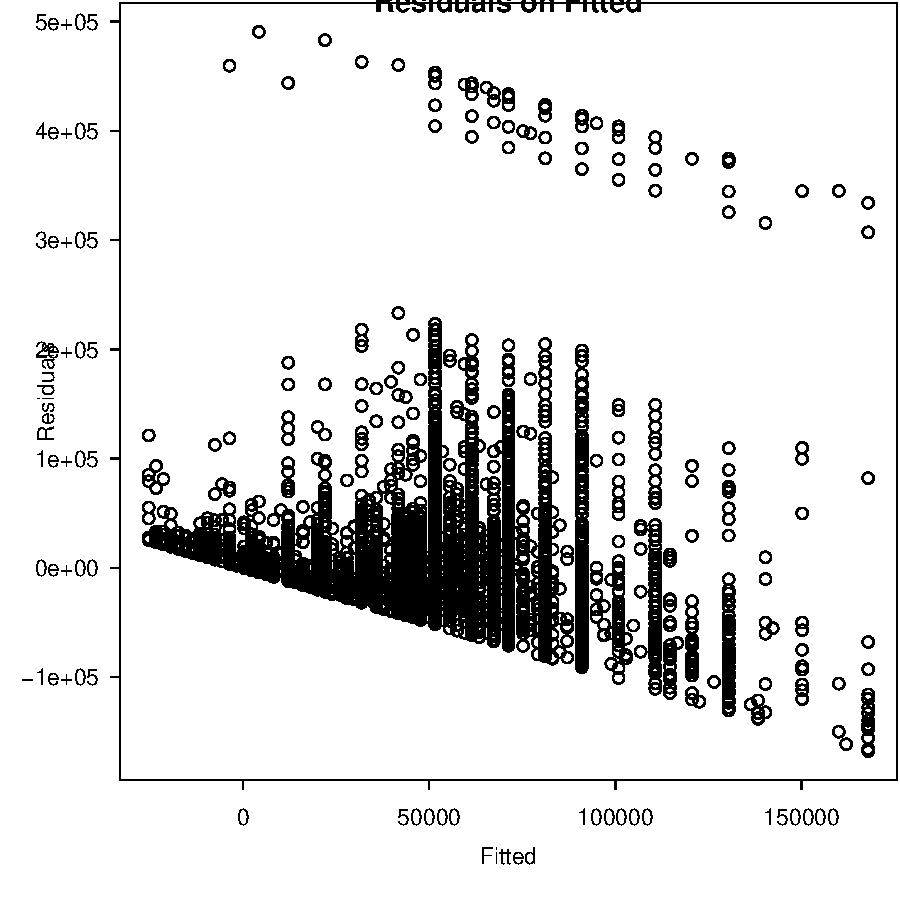
\includegraphics[width=.6\linewidth]{figure/HW0-Final-Rnwauto-report-1} 

}


\begin{kframe}\begin{alltt}
\hlkwd{ggplot}\hlstd{(mtcars)}\hlopt{+} \hlkwd{geom_point}\hlstd{(}\hlkwc{mapping} \hlstd{=} \hlkwd{aes}\hlstd{(}\hlkwc{x} \hlstd{= mpg,} \hlkwc{y} \hlstd{= wt,}
                                         \hlkwc{color} \hlstd{= mtcars}\hlopt{$}\hlstd{am,}
                                         \hlkwc{shape} \hlstd{= mtcars}\hlopt{$}\hlstd{gear))} \hlopt{+} \hlkwd{scale_shape_identity}\hlstd{()} \hlopt{+}
  \hlkwd{labs}\hlstd{(}\hlkwc{title} \hlstd{=} \hlstr{"Weight on Miles per Gallon"}\hlstd{,} \hlkwc{x} \hlstd{=} \hlstr{"Miles per Gallon"}\hlstd{,} \hlkwc{y} \hlstd{=} \hlstr{"Weight"}\hlstd{)} \hlopt{+}
  \hlkwd{theme}\hlstd{(}\hlkwc{panel.background} \hlstd{=} \hlkwd{element_rect}\hlstd{(}\hlkwc{fill} \hlstd{=} \hlstr{"lightyellow"}\hlstd{))}
\end{alltt}
\end{kframe}

{\centering 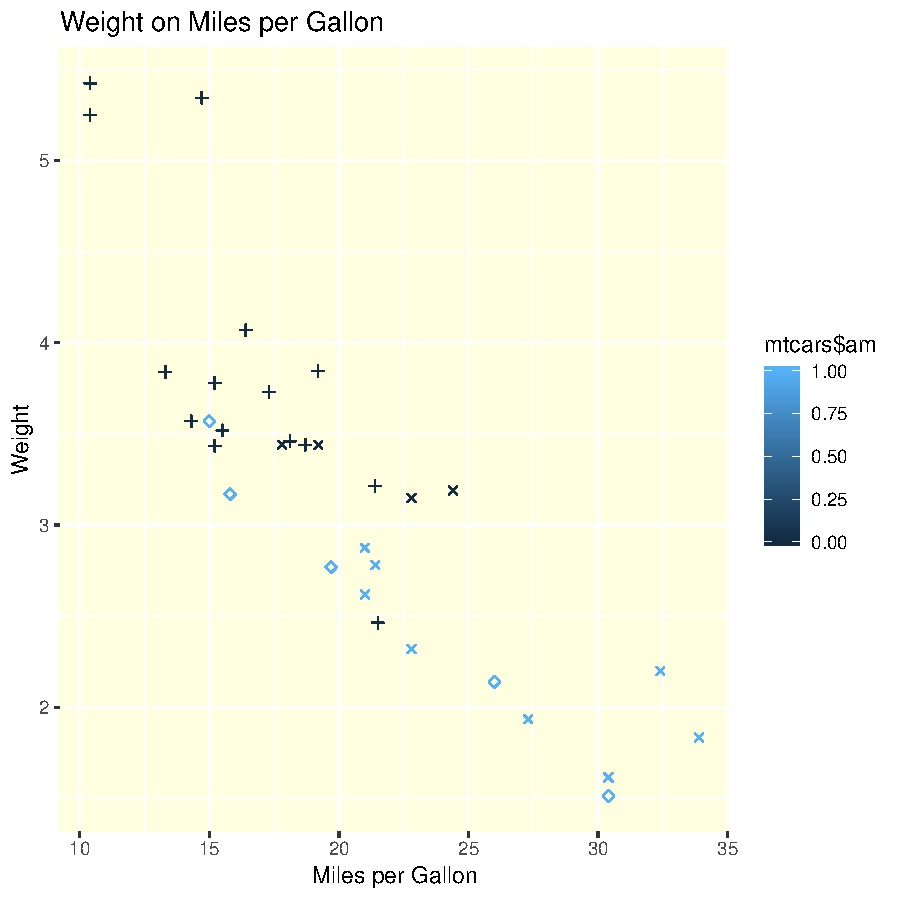
\includegraphics[width=.6\linewidth]{figure/HW0-Final-Rnwauto-report-2} 

}



\end{knitrout}

The R session information (including the OS info, R version and all
packages used):

\begin{knitrout}
\definecolor{shadecolor}{rgb}{0.969, 0.969, 0.969}\color{fgcolor}\begin{kframe}
\begin{alltt}
\hlkwd{sessionInfo}\hlstd{()}
\end{alltt}
\begin{verbatim}
## R version 3.5.3 (2019-03-11)
## Platform: x86_64-w64-mingw32/x64 (64-bit)
## Running under: Windows >= 8 x64 (build 9200)
## 
## Matrix products: default
## 
## locale:
## [1] LC_COLLATE=English_United States.1252  LC_CTYPE=English_United States.1252   
## [3] LC_MONETARY=English_United States.1252 LC_NUMERIC=C                          
## [5] LC_TIME=English_United States.1252    
## 
## attached base packages:
## [1] stats     graphics  grDevices utils     datasets  methods   base     
## 
## other attached packages:
## [1] ggplot2_3.1.1  gmodels_2.18.1 knitr_1.22    
## 
## loaded via a namespace (and not attached):
##  [1] Rcpp_1.0.1       magrittr_1.5     MASS_7.3-51.1    tidyselect_0.2.5 munsell_0.5.0   
##  [6] colorspace_1.4-1 R6_2.4.0         rlang_0.3.3      dplyr_0.8.0.1    stringr_1.4.0   
## [11] highr_0.8        plyr_1.8.4       tools_3.5.3      grid_3.5.3       gtable_0.3.0    
## [16] xfun_0.6         withr_2.1.2      gtools_3.8.1     digest_0.6.18    assertthat_0.2.1
## [21] yaml_2.2.0       lazyeval_0.2.2   tibble_2.1.1     crayon_1.3.4     purrr_0.3.2     
## [26] glue_1.3.1       evaluate_0.13    labeling_0.3     gdata_2.18.0     stringi_1.4.3   
## [31] compiler_3.5.3   pillar_1.3.1     scales_1.0.0     pkgconfig_2.0.2
\end{verbatim}
\begin{alltt}
\hlkwd{Sys.time}\hlstd{()}
\end{alltt}
\begin{verbatim}
## [1] "2019-04-13 18:14:45 CDT"
\end{verbatim}
\end{kframe}
\end{knitrout}


\end{document}
